\section{SVD-LLM V2}
\label{sec:methodology}

% \begin{figure*}[t]
% \centering
% 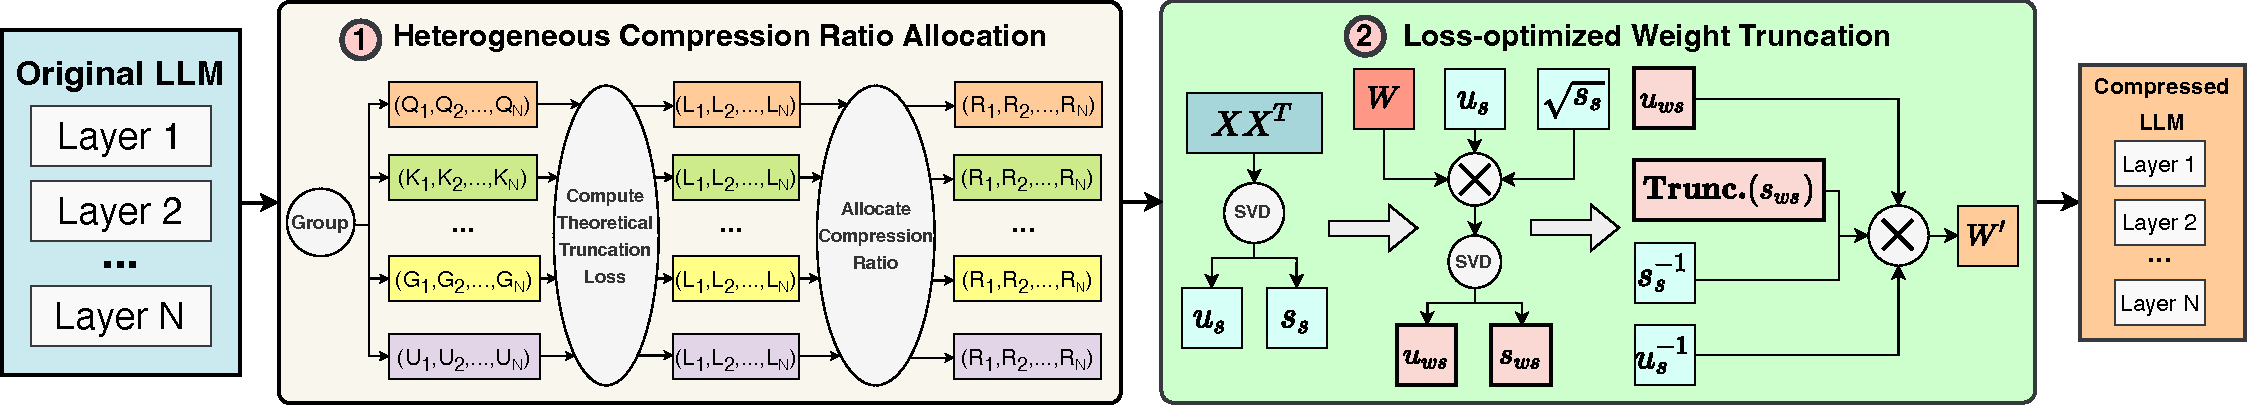
\includegraphics[width=1\textwidth]{Figures/Framework.pdf}
% \caption{Overview of \sysname.}
% \label{fig:framework}
% \end{figure*}

% \begin{figure}[htbp]
%     \centering
%     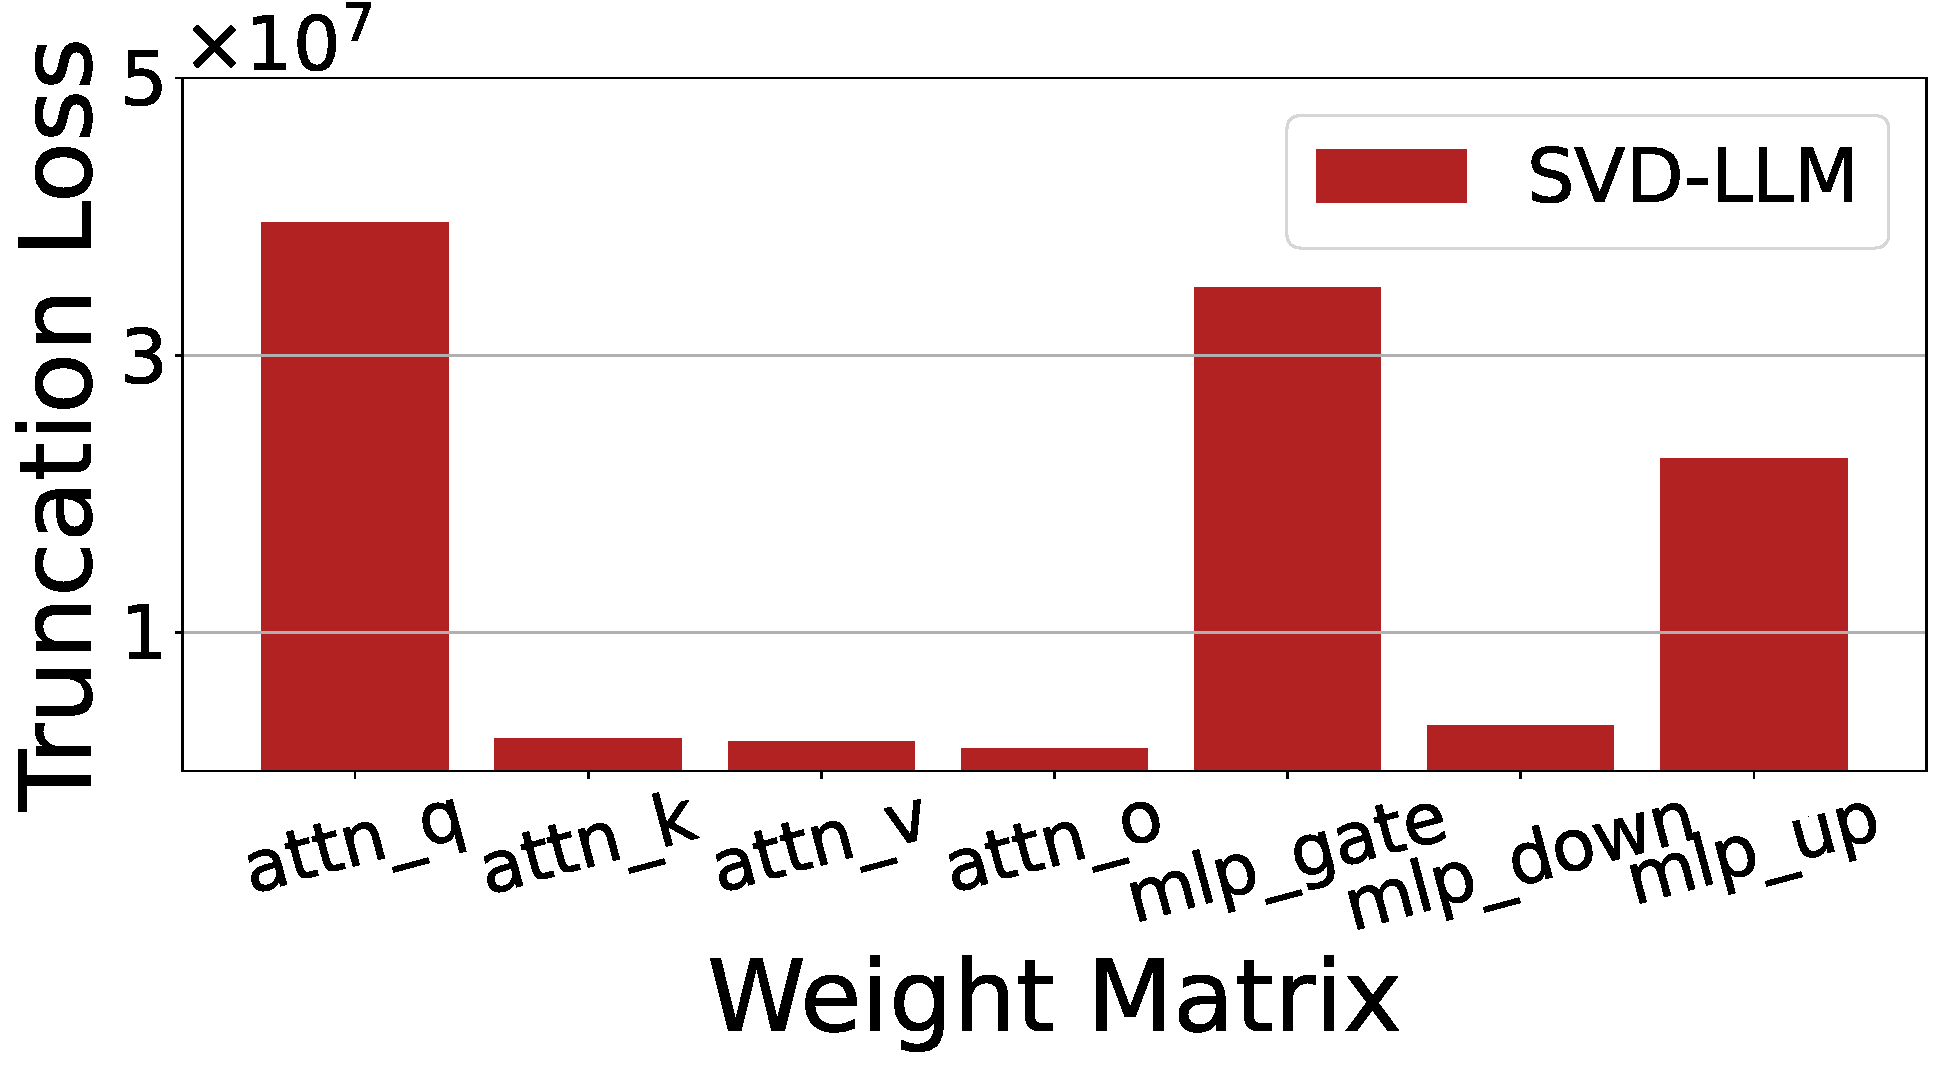
\includegraphics[width=0.45\textwidth]{Figures/Motivation_2.pdf}
%     \caption{Truncation loss by SVD-LLM of weight matrices in one randomly selected decoding layer in LLaMA-3 8B on WikiText-2 under 50\% compression ratio.}
%     \label{fig:motivation_2}
% \end{figure}

%In this section, we present the main design of our proposed \sysname for compressing LLMs. 
\cref{fig:framework} provides an overview of \sysname. 
%
Specifically, \sysname groups the weight matrices across all the layers in the original LLM by type, such as query ($Q$) and key ($K$) in attention blocks, and Gate ($G$) and Up ($U$) in MLP blocks. It then computes the theoretical truncation loss of the weight matrices and assigns a unique compression ratio to each weight matrix within each group based on the computed truncation loss.
%After obtaining all compression ratios across the weight matrices, 
Lastly, \sysname performs loss-optimized weight truncation to obtain the compressed LLM.
%
Below, we describe the details of the two main components of \sysname: (1) heterogeneous compression ratio allocation and (2) loss-optimized weight truncation. 
%
% The pseudocode of \sysname is provided in \xin{xxx}.

% \subsection{Motivation}
% \label{subsec:motivation}
% % \xin{Loss figure (loss increases significantly with ratio}
% To ensure better compression performance, many recent post-training SVD-based LLM compression works~\citep{DBLP:conf/iclr/HsuHCLSJ22, DBLP:journals/corr/abs-2312-05821, DBLP:journals/corr/abs-2403-07378} attempt to lower the truncation loss $L$ in the form of Frobenius norm as follows during their LLM compression:

% \begin{equation}
%     L = ||WX-W'X||_F 
%     \label{eq:t1}
% \end{equation}

% \noindent where $W$ is the weight matrix of the original LLM, $X$ is the activation of $W$, and $W'$ is the compressed low-ranking weight matrix.

% Although the state-of-the-art method SVD-LLM~\citep{DBLP:journals/corr/abs-2403-07378} has theoretically guaranteed the alignment between truncated singular values and the corresponding truncation loss, which reduces the truncation loss and significantly enhances the compressed LLMs' performance, it still fails to ensure the minimization of the truncation loss during the SVD compression. 
% %
% For a better demonstration, we randomly select one of the decoding layers in LLaMA-3 8B and compute the corresponding truncation loss of all weight matrices under 50\% compression ratio. As shown in~\cref{fig:motivation_2}, all the weight matrices suffer severely from the huge truncation loss. For the weight matrices in other decoding layers, we also observe a similar trend.
% %
% As a result, the output $W'X$ computed by the compressed weight matrix $W$ significantly deviates from $WX$ computed by the original weight matrix $W$, causing the final performance of compressed LLM to drop significantly. Therefore, it is still necessary to design a new method with a better ability to minimize truncation loss.

\subsection{Heterogeneous Compression Ratio Allocation}
\label{subsec:dynamic_ratio_allocation}
\noindent \textbf{Motivation:} Since different weight matrices in LLMs often exhibit different levels of redundancy, applying a homogeneous compression ratio to all the weight matrices would incur high truncation loss for those with low redundancy~\citep{DBLP:journals/corr/abs-2406-10594,DBLP:journals/corr/abs-2406-15786,DBLP:journals/corr/abs-2407-19126}. 
%
To demonstrate this, we use SVD-LLM to measure the truncation loss of the query matrix across different layers in LLaMA-3 8B on WikiText-2 dataset with 50\% compression ratio. 
%
As shown in~\cref{fig:layer}, the truncation loss varies at different layers. For example, the query matrix in the 27th layer has a much higher truncation loss than that of the first layer, indicating the 27th layer should be compressed under a smaller compression ratio, while a larger compression ratio should be applied to the first layer. 
%
However, existing SVD-based LLM compression methods either overlook this variation or require resource-intensive operations to determine the specific compression ratios, making them impractical for compressing LLMs at larger scales. 
%
Therefore, it is essential to develop a more efficient approach to apply different compression ratios at different weight matrices to reduce the truncation loss.


\begin{figure}[t]
    \centering
    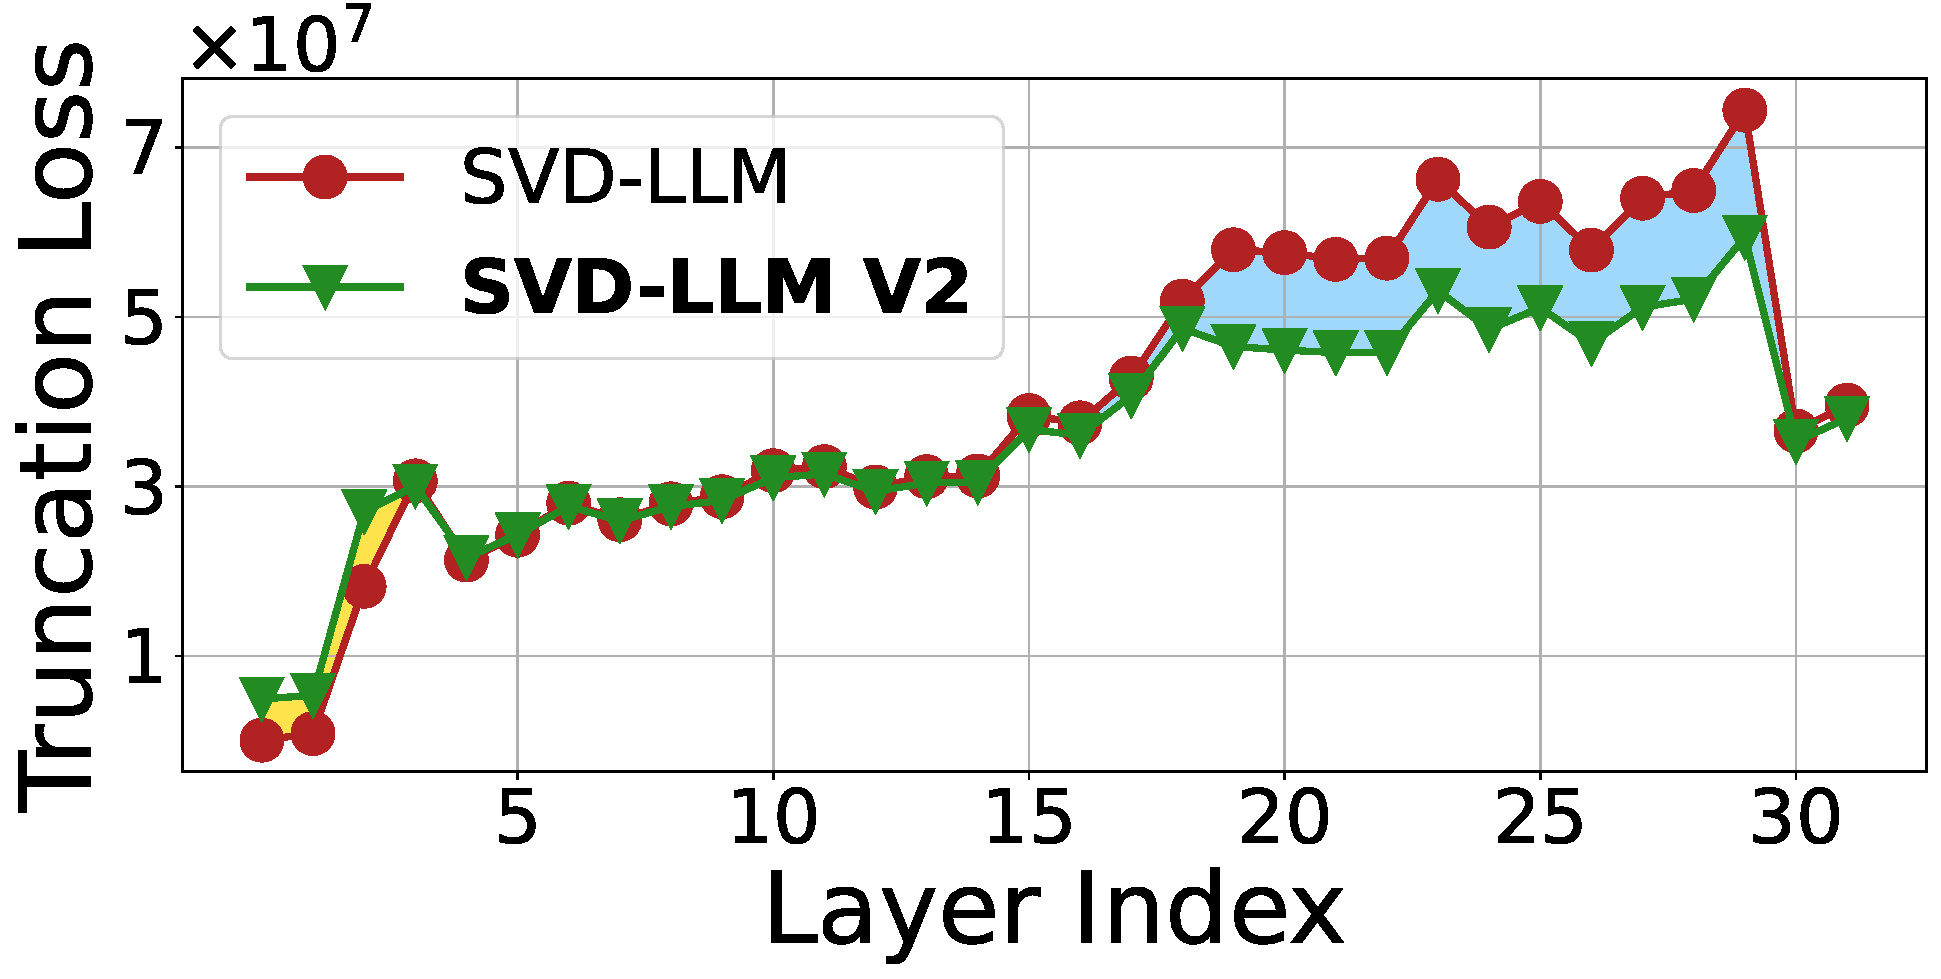
\includegraphics[width=0.45\textwidth]{Figures/Layer.pdf}
    \caption{Comparison between SVD-LLM and \sysname on the truncation loss of the query weight matrix across different layers in LlaMA-3 8B on WikiText-2 dataset with 50\% compression ratio.}
    \label{fig:layer}
\end{figure}


\begin{algorithm}[t]
\captionsetup{font=small}
\caption{Pseudocode of Heterogeneous Compression Ratio Allocation in \sysname}
\small
\begin{algorithmic}[1] % The number [1] tells LaTeX to number each line
\Statex \textbf{Input:} $M$: Original LLM 
\Statex \hspace{3em} $x$: Input activation
\Statex \hspace{3em} $R$: Target compression ratio
\Statex \textbf{Output:} $R_d$: A list of allocated compression ratios
% \setcounter{ALG@line}{0}  % 重置行号计数器，从0开始
\Procedure{Ratio\_Allocation}{$M, S, R$} % Algorithm name and parameters
    \State $G \gets \boldsymbol{\operatorname{Group}}(M)$  \Comment{Group the weight by types}
    \State $R_d \gets \emptyset$ \Comment{Initialize the compression ratio list} 
        \For{$g$ \textbf{in} $G$}
        \State $L_G \gets \emptyset$ \Comment{Initialize the loss list in the group} 
            \For{$w$ \textbf{in} $g$}
            % \State $w' \gets \boldsymbol{\operatorname{Weight\_Truncation}}(w, x, R)$
                \State $L_{min} \gets \boldsymbol{\operatorname{Theoretical\_Loss}}(w, x, R)$
                \State $L_{G} \gets L_{G} \cup L_{min}$ 
            \EndFor
            \State $L_{G} \gets 1 / \boldsymbol{\operatorname{Log}}(L_{G})$ \Comment{Normalize $L_G$}
            \State $r \gets \boldsymbol{\operatorname{Len}}(L_{G}) \times R\times L_{min} / \boldsymbol{\operatorname{Sum}}(L_{G})$
            \State $R_d \gets R_d \cup r$ \Comment{Append $r$ to the list $R_d$} 
        \EndFor
    \State \Return{$R_d$}
\EndProcedure
\end{algorithmic}
\label{algo:compression_ratio}
\end{algorithm}

\noindent \textbf{Key Design:} 
%
The pseudocode of the heterogeneous compression ratio allocation is listed in~\cref{algo:compression_ratio}. 
%
Specifically, 
% to calculate the truncation loss more efficiently and accurately, 
% \sysname applies a whitening matrix $S$,  as done in SVD-LLM~\citep{DBLP:journals/corr/abs-2403-07378} to align the truncation loss with singular values. 
% We follow the same procedure in SVD-LLM to construct a calibration set $X$ and compute the whitening matrix $S$ with the Choloesky decompostion of $XX^T$. In this way, the truncation loss $L$ to truncate the multiple singular values $(\sigma_0, \sigma_1, \cdots, \sigma_k)$ could easily be obtained by $\sqrt{\sum_{i=0}^k \sigma_i^2}$. 
% \sysname applies its own loss-optimized weight truncation, which is more accurate and stable than the truncation done in SVD-LLM, as described in~\cref{subsec:loss_optimized_weight_truncation} to pre-compress the weight matrix under a given compression ratio $R$ and compute its corresponding truncation loss.
%
given that different types of weight matrices, such as query ($Q$) and key ($K$) in attention blocks, and Gate ($G$) and Up ($U$) in MLP blocks play different roles in an LLM, 
%it is inappropriate to consider them together for compression ratio allocation. 
%Therefore, given the specific compression ratio $R$, 
\sysname first groups the weight matrices across all the layers in the original LLM according to their types. 
%
Next, \sysname computes the theoretical minimum truncation loss of the weight matrices, i.e., $L_{min} = ||C-C'||_F$, where $C$ is the original matrix of $WX$ and $C'$  is its compressed version by SVD, respectively. It then inverses and normalizes $L_{min}$ by $1/\text{Log}(L_{min})$.
%
Finally, given the target model compression ratio $R$, the compression ratio of each weight matrix within a group is determined as $ \text{Len}(L_{G}) \times R \times L_{min} / \text{Sum}(L_{G})$, where $L_{G}$ denotes the list of theoretical truncation loss for all matrices within the same group, $\text{Len}(L_{G})$ denotes the group size and $\text{Sum}(L_{min})$ denotes the sum of the loss within this group. 
%
In this way, \sysname bypasses the need to measure end-to-end perplexity to determine compression ratios, as done in ASVD and is time-consuming. Instead, it utilizes truncation loss, which is easy to obtain and thereby enhancing the efficiency of the algorithm.
%
As shown in~\cref{fig:layer}, with the proposed heterogeneous compression ratio allocation scheme, \sysname effectively reduces the truncation loss (the blue area) with only a small increase of several small truncation losses (the yellow area).

% After determining the specific compression ratio for each weight matrix in the LLM, \sysname incorporates a loss-optimized weight truncation to truncate the weight matrices based on their assigned compression ratios to obtain the compressed LLM.
%the next step is to apply the real truncation on the weights  
%
In the next section, we describe the details of the proposed loss-optimized weight truncation.  
%
% \vspace{-3mm}



\subsection{Loss-optimized Weight Truncation}
\label{subsec:loss_optimized_weight_truncation}
%
\noindent \textbf{Motivation:} 
After determining the specific compression ratio for each weight matrix in the LLM, the next step is to truncate the weights according to their assigned compression ratios. 
%
To reduce truncation loss $L= ||WX-W'X||_F$ during SVD compression, SVD-LLM first constructs the whitening matrix $S$ by applying Cholesky decomposition on $XX^T$. It then performs SVD and truncation on $WS$. Although SVD-LLM has been theoretically proven to achieve the lowest truncation loss at a given compression ratio, our empirical study shows that its actual truncation loss is frequently above the theoretical minimum. This is mainly due to the numerical instability involved in performing the Cholesky decomposition on a large-scale matrix during truncation. Moreover, the Cholesky decomposition requires $XX^T$ to be positive definite, which is often hard to satisfy.
%during compression.

%
To demonstrate this, we randomly select two weight matrices, $A$ and $B$, in LLaMA-3 8B and compute their truncation loss by SVD-LLM using 256 randomly selected data in the C4 dataset under compression ratios 20\% and 60\%. As shown in~\cref{tab:loss_comparison}, because $XX^T$ is not positive definite, SVD-LLM fails to compress matrix $A$. For matrix $B$, even when the compression ratio is as low as 20\%, SVD-LLM still achieves a larger truncation loss in practice than in theory, and this difference even increases with increasing compression ratio. 

SVD-based LLM compression methods such as Balco~\citep{DBLP:journals/corr/abs-2405-10616} have been proposed that utilize pooled covariance matrices to precisely estimate the feature distribution to reduce truncation loss. However, these methods cannot guarantee their theoretical optimality during SVD truncation. 
%
Therefore, it is necessary to design a new way to optimize the truncation loss for SVD compression. 

\losscomparisonTable
\vspace{2mm}

% \begin{figure}[htbp]
%     \centering
%     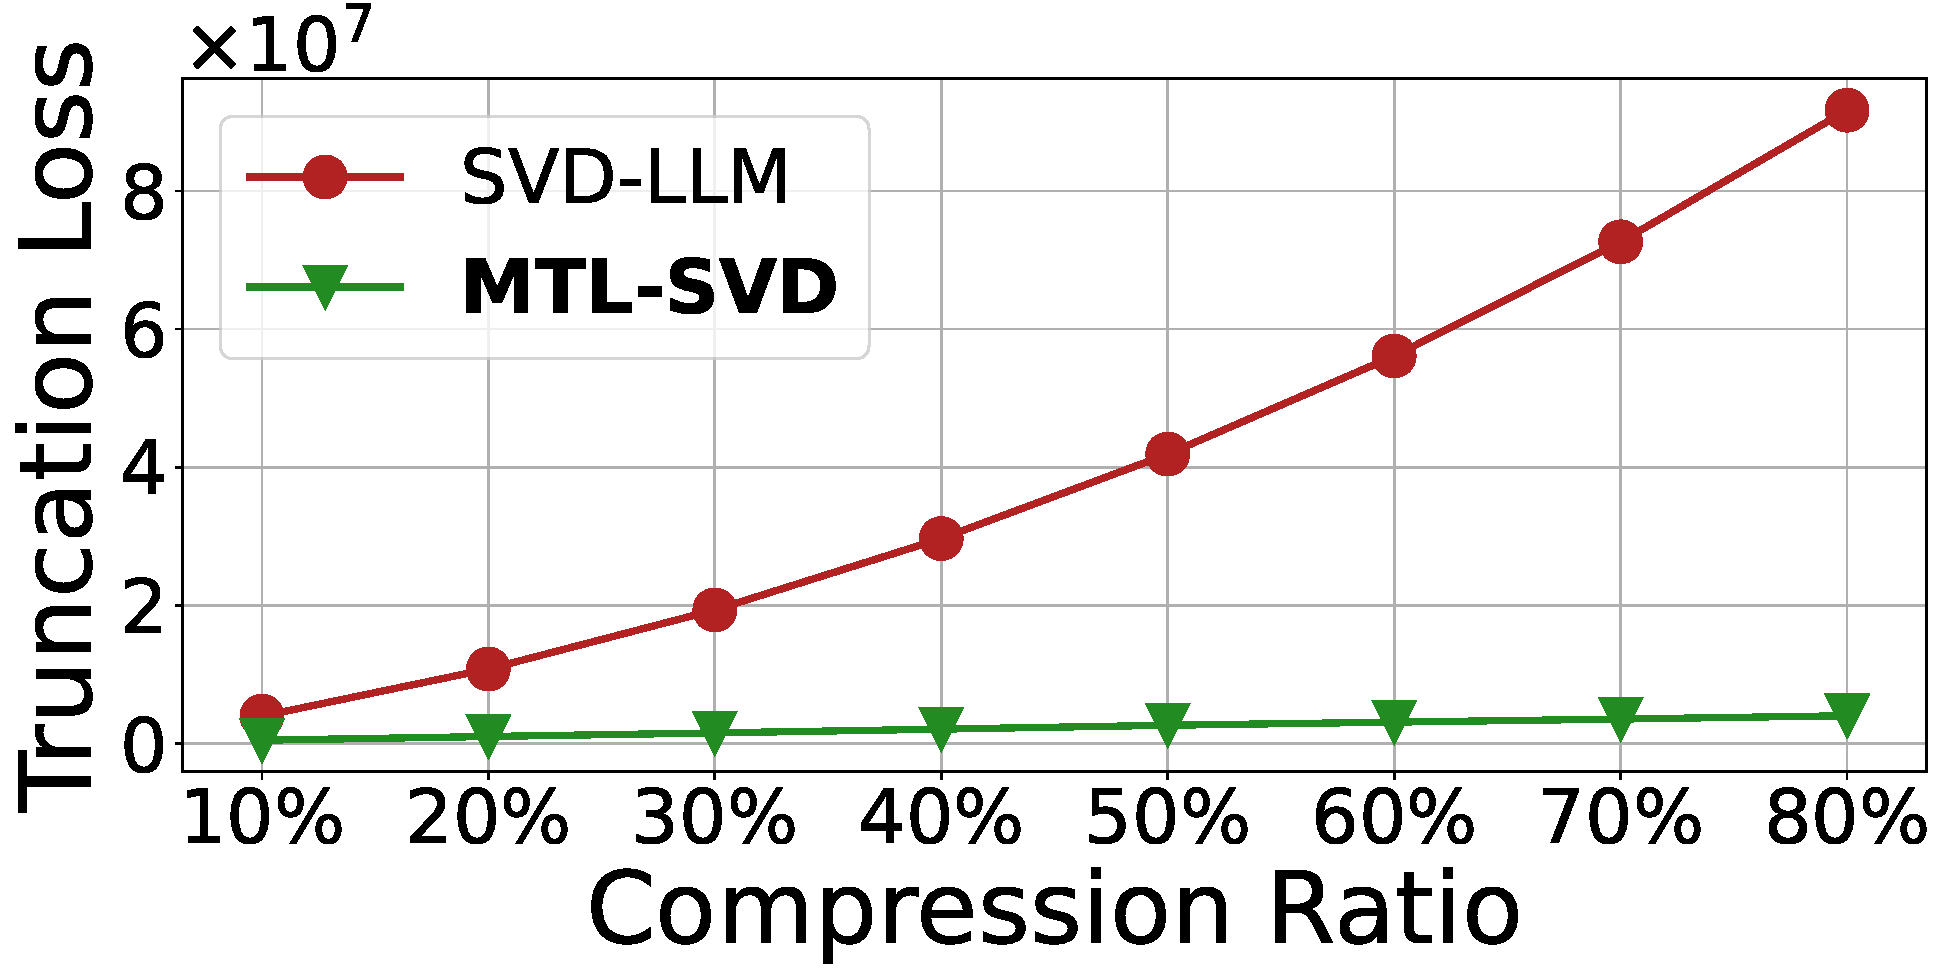
\includegraphics[width=0.45\textwidth]{Figures/Loss.pdf}
%     \caption{Truncation loss by SVD-LLM and \sysname of the weight matrix randomly selected in LLaMA-3 8B on WikiText-2 under different compression ratios.}
%     \label{fig:loss}
% \end{figure}

\begin{algorithm}[t]
\captionsetup{font=small}
\caption{Pseudocode of Loss-optimized Weight Truncation in \sysname}
\small
\begin{algorithmic}[1] % The number [1] tells LaTeX to number each line
\Statex \textbf{Input:} $W$: Original weight matrix 
\Statex \hspace{3em} $X$: Input activation
\Statex \hspace{3em} $R$: Target compression ratio
\Statex \textbf{Output:} $W'$: Compressed weight matrix
% \setcounter{ALG@line}{0}  % 重置行号计数器，从0开始
\Procedure{Weight\_Truncation}{$W, X, R$} % Algorithm name and parameters
    \State $S \gets XX^T$  \Comment{Construct matrix $S$ from $X$}
    \State $U_s, S_s, V_s \gets \boldsymbol{\operatorname{SVD}}(S)$ \Comment{Perform SVD on matrix $S$} 
    \State $D \gets W\times U_s \times \sqrt{S_s}$  \Comment{Construct matrix $D$}
    \State $U_{ws}, S_{ws}, V_{ws} \gets \boldsymbol{\operatorname{SVD}}(D)$ \Comment{Perform SVD on matrix $D$}
    \State $T_s \gets \boldsymbol{\operatorname{Truncate}}(S_{ws}, R)$ \Comment{Perform SVD truncation on matrix $S_{ws}$ based on compression ratio $R$}
    \State $W' \gets U_{ws}\times T_s \times S_{s} ^{-1}\times U_{s}^{-1}$ \Comment{Construc $W'$}
    \State \Return{$W'$}
\EndProcedure
\end{algorithmic}
\label{algo:weight_truncation}
\end{algorithm}




\noindent \textbf{Key Design:}
The pseudocode of the proposed loss-optimized weight truncation is provided in~\cref{algo:weight_truncation}. Different from SVD-LLM, \sysname bypasses the Cholesky decomposition, resulting in a more straightforward process with improved numerical stability. Specifically, given the input activation $X$, \sysname conducts SVD on $XX^T$ to obtain the decomposed matrices $U_s, S_s, V_s$, where $S_s$ is the diagonal matrix with singular values. It then conducts another round of SVD on $W\times U_s\times \sqrt{S_s}$ to obtain $U_{ws}, S_{ws}, V_{ws}$. The final compressed weight matrix $W'$ can be obtained via $U_{ws}\times \boldsymbol{\operatorname{Trunc.}}(S_{ws}) \times S_{s} ^{-1}\times U_{s}^{-1} $, where $\boldsymbol{\operatorname{Trunc.}}(C)$ denotes the rank-k truncation of matrix $C$ during SVD compression.

In the following, we provide a theoretical proof on why such truncation offers the same theoretical minimum truncation loss as SVD-LLM.

\begin{theorem}
\label{thm:whitening}
If $U_s, S_s, V_s$ are obtained by SVD decomposition of $XX^T$ and $U_{ws}, S_{ws}, V_{ws}$ are obtained by SVD decomposition of $W\times U_s\times \sqrt{S_s}$, the compressed weight matrix $W' = U_{ws}\times \boldsymbol{\operatorname{Trunc.}}(S_{ws}) \times V_{ws} \times \sqrt{S_{s}}^{-1} \times U_{s}^{-1}$ ensures the theoretical minimum truncation loss.
\end{theorem}

\begin{proof}
\label{proof:truncation}
Since $XX^T$ is the symmetric matrix, suppose that the singular vectors and values of input activation $X$ is $U_x, S_x, V_x$, we have $U_s = U_x$ and $\sqrt{S_s} = S_x$. Suppose $S = U_s\times \sqrt{S_s}$, thus $S^{-1} = \sqrt{S_{s}}^{-1} \times U_{s}^{-1}$, and we have:

 % \vspace{-2mm}
{\small
\begin{equation}
    \begin{aligned}
        &S^{-1} X = \sqrt{S_{s}}^{-1} U_{s}^{-1} X = S_{x}^{-1} U_{x}^{-1} X\\
        &= S_{x}^{-1} U_{x}^{-1} U_x S_x V_x = Vx
    \end{aligned}
\label{formula:derive}
\end{equation}
}

\noindent Therefore, $S^{-1}\times X$ is orthogonal and $||A\times S^{-1}\times X||_F = ||S^{-1}\times X||_F$, and the final truncation loss could be derived as:

%\vspace{-4mm}
{\small
\begin{equation}
    \begin{aligned}
        &L^2 =||W X-W^{\prime} X||_F^2 \\
        &= ||WSS^{-1}X - U_{ws}\times \boldsymbol{\operatorname{Trunc.}}(S_{ws}) \times V_{ws} \times S^{-1} X||_F^2\\
        &= ||(WS - U_{ws}\times \boldsymbol{\operatorname{Trunc.}}(S_{ws}) \times V_{ws})S^{-1}X||_F^2\\
        &= ||WS - U_{ws}\times \boldsymbol{\operatorname{Trunc.}}(S_{ws}) \times V_{ws}||_F^2\\
        &= ||\boldsymbol{\operatorname{SVD}}(WS)||_F^2 = ||\boldsymbol{\operatorname{SVD}}(W\times U_x\times S_x)||_F^2\\
        & = ||\boldsymbol{\operatorname{SVD}}(W\times U_x\times S_x\times V_x)||_F^2\\
        & = ||\boldsymbol{\operatorname{SVD}}(WX)||_F^2 = L_{min} ^2
    \end{aligned}
\label{formula:loss_1}
\end{equation}
}

\noindent Therefore, the designed SVD truncation ensures the theoretical minimum truncation loss.
\end{proof}

For a better demonstration, we also implement the new loss-optimized weight truncation by \sysname on LLaMA-3-8B. As shown in~\cref{tab:loss_comparison}, \sysname achieves better numerical stability and lower truncation loss than SVD-LLM.
% demonstrating the effectiveness of our proposed loss-minimized weight truncation strategy.

% \noindent Therefore, we have: 

% % \vspace{-2mm}
% {\small
% \begin{equation}
%     \begin{aligned}
%         &L^2 =||W X-W^{\prime} X||_F^2 \\
%         & =\sum_{j=1}^r \sum_{i=1}^r \sigma_i \sigma_j \boldsymbol{\operatorname{trace}}(Mu_i v_i^T v_j u_j^TM^T)\\
%         & =  \sum_{i=1}^r\sigma_i^2\boldsymbol{\operatorname{trace}}(Mu_iu_i^TM^T)\\
%         & =  \sum_{i=1}^r\sigma_i^2||Mu_i||_F^2 \leq ||M||_F^2\sum_{i=1}^r\sigma_i^2
%     \end{aligned}
% \label{formula:loss_2}
% \end{equation}
% }

% \noindent Therefore, we have $L\leq\sqrt{||M||_F^2\sum_{i=1}^r \sigma_i^{2} }$.


% Therefore, we could  indirectly minimize the truncation loss through lowering this upper-bound. The gradient of $L$ can be calculated as:

% % \vspace{-4mm}
% {\small
% \begin{equation}
%     \begin{aligned}
%         &\nabla_M L^2=\nabla_M (||M||_F^2\cdot \sum_{i=1}^r\sigma_i^2)\\
%         &=\nabla_M||M||_F^2\cdot \sum_{i=1}^r\sigma_i^2 + ||M||_F^2 \nabla_M\sum_{i=1}^r\sigma_i^2\\
%         &=\sum_{i=1}^r\sigma_i^2 \cdot 2M - 2||M||_F^2 \cdot \sum_{i=1}^r\sigma_i (M^{-1})^TU_iV_i^T(WS)^T
%     \end{aligned}
% \label{formula:gradient}
% \end{equation}
% }

% \noindent where $U_i$ and $V_i$ are the left and right singular vectors corresponding to the $i$-th singular value $\sigma_i$. Therefore, the gradient is easy to obtain, which makes it convenient for us to apply some existing optimization algorithms\footnote{In our paper, we use L-BFGS~\citep{Nash1991ANS} algorithms as the default} with the computed gradient to further minimize the truncation loss. Different from directly optimizing $W'$ based on the original truncation loss $L = ||WX-W'X||_F$ that requires storing every large-scale activation matrix $X$, which is impractical in the post-training LLM compression scenario, optimizing with gradient computed from \cref{formula:gradient} does not need to store activation, which is more efficient and feasible.

% \begin{figure}[htbp]
% % \vspace{-2mm}
%     \centering
%     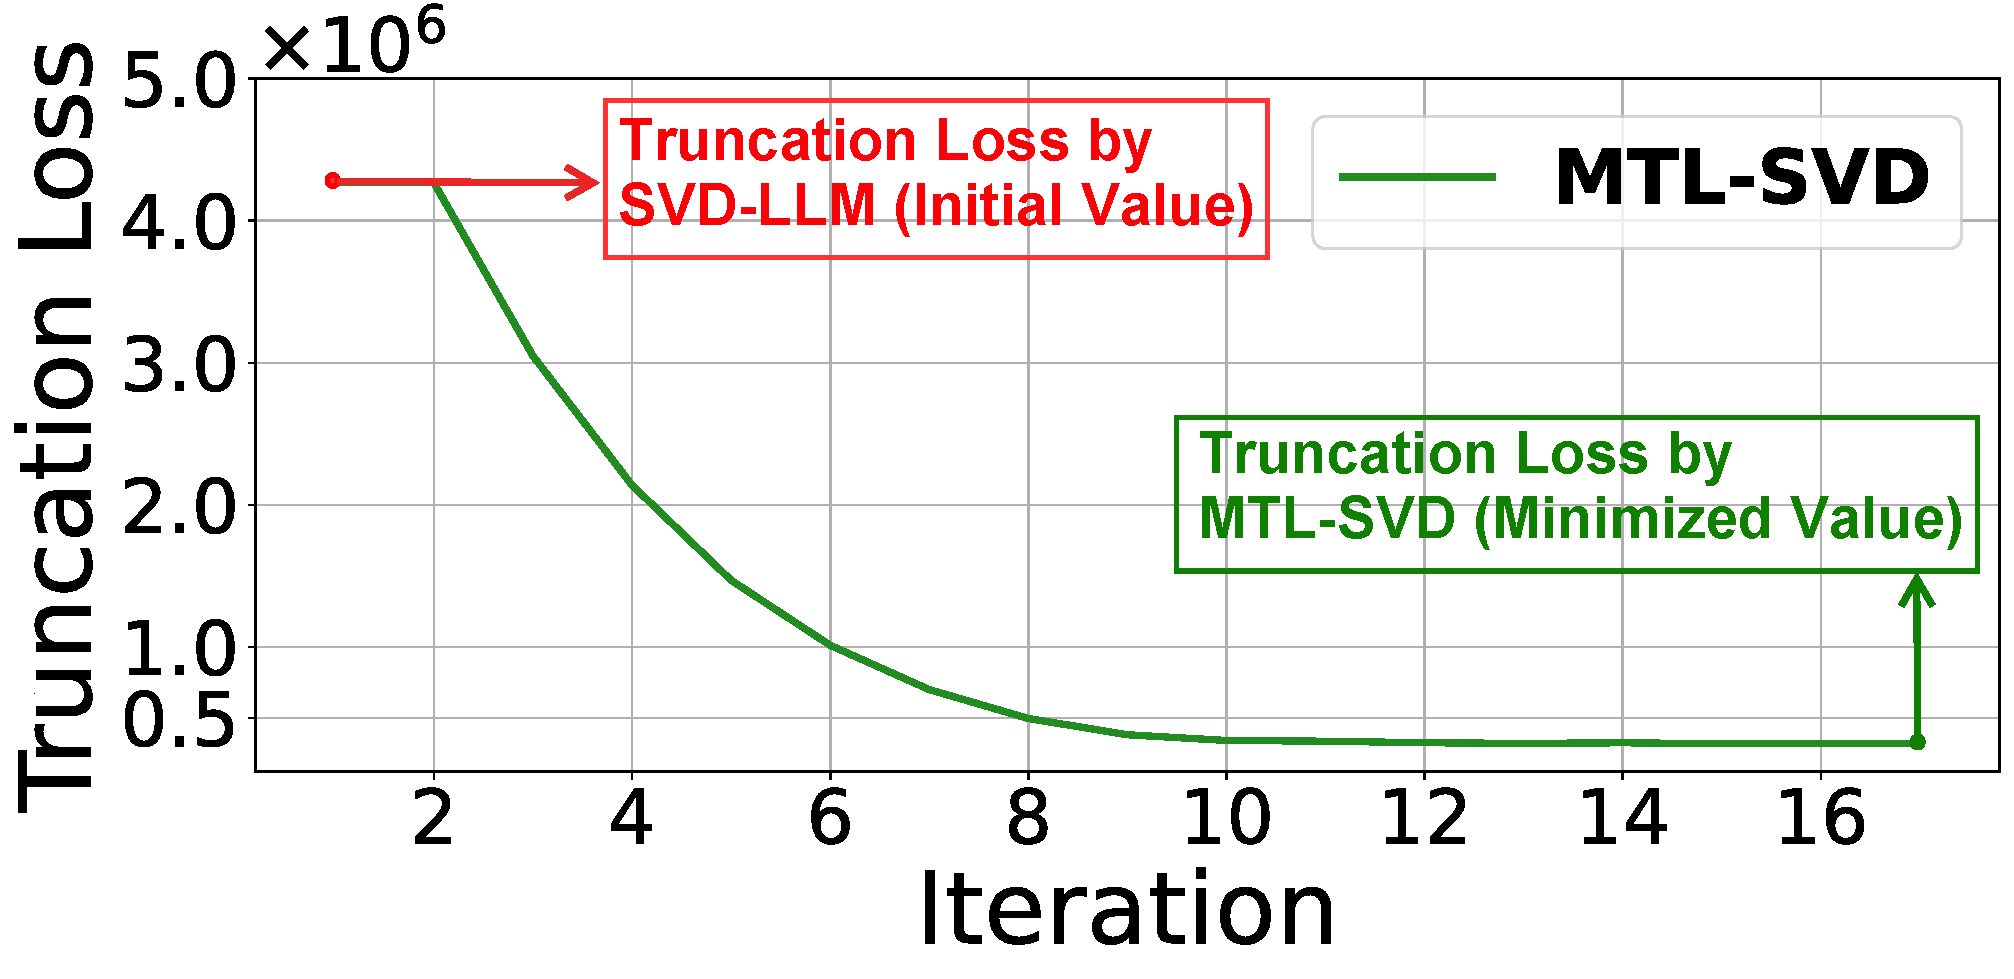
\includegraphics[width=0.45\textwidth]{Figures/Gradient.pdf}
%     \caption{Truncation loss (upper-bound) of the weight matrix in LLaMA-3 8B during the optimization process.}
%     \label{fig:gradient}
%     % % \vspace{-2mm}
% \end{figure}

% To further improve the optimization efficiency, we initialize $M$ to identity matrix, i.e., $M = I$. Therefore, the initial truncation loss is $\sqrt{\sum_{i=1}^r\sigma_i^2}$, which is exactly equal to the truncation loss obtained by SVD-LLM. For a better demonstration, we randomly select one weight matrix in LLaMA-3 8B and plot its upper-bound truncation loss during the optimization process. As shown in~\cref{fig:gradient}, the truncation loss drops significantly via optimization, 
% demonstrating the effectiveness of our proposed loss-minimized weight truncation strategy.

